Since the beginning of modern biology, gene expression is part of the central dogma of molecular biology.
Of course, during the decades some aspects have changed, but the \gls{rna} transcripts still have very high relevance.
Nowadays, \textit{RNA-seq} \cite{Thermes2014, Wang2009, Costa2010, Ozsolak2011} is the most widely used technology to understand gene related regulatory mechanisms in response to stress conditions or drug treatments and progressions of several diseases \cite{Costa2013}.

The main aim of \textit{RNA-seq} experiment is to highlight which genes are increasingly (\textit{up-regulated}) or decreasingly (\textit{down-regulated}) altered when comparing two or more conditions at a specific instant in time or in subsequent time points (time-course experiment), and then identify the biological mechanisms regulating such changes.

However, \textit{RNA-seq} also offers the possiblity to identify and investigate isoforms abundance \cite{Trapnell2010, Roberts2011, Roberts2011a, Trapnell2013}.
Although, such aspect will not be further treated in this thesis.

The general idea underlying the library preparation of an \textit{RNA-seq} experiment can be viewed as the conversion of long \glspl{mrna} segments in \gls{cdna} fragments with \gls{rna} or \gls{dna} fragmentation. 
To each sequence, an adapter for the sequencer is added and a short read is obtained with high-throughput sequencing technology (Figure \ref{fig:rnaseqexp}).

\begin{figure}[h]
\centering
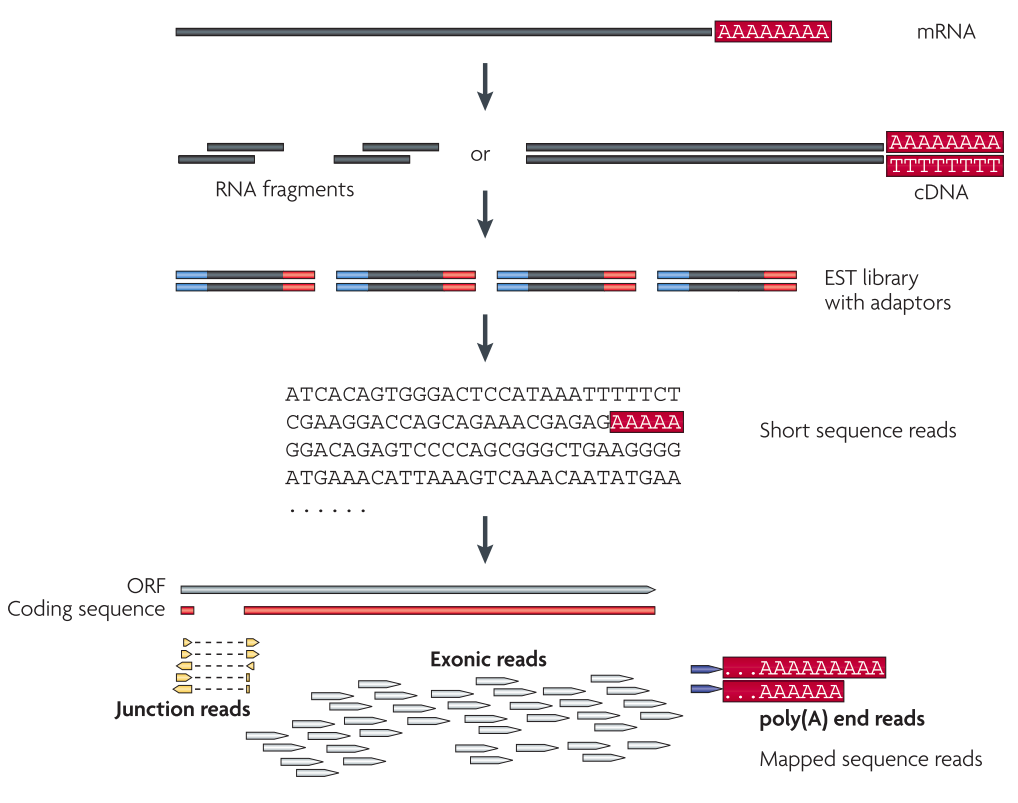
\includegraphics[width=9cm, keepaspectratio]{img/intro/rna-seq.png}
\caption[RNA-seq experiment]{Representation of an RNA-seq experiment. \cite{Wang2009}}
\label{fig:rnaseqexp}

\end{figure}

Afterwards, the so-obtained reads need to be analyzed with several tools, depending on the particular question the researcher is interested in \cite{Pepke2009, Oshlack2010}.

\begin{figure}[h]
\centering
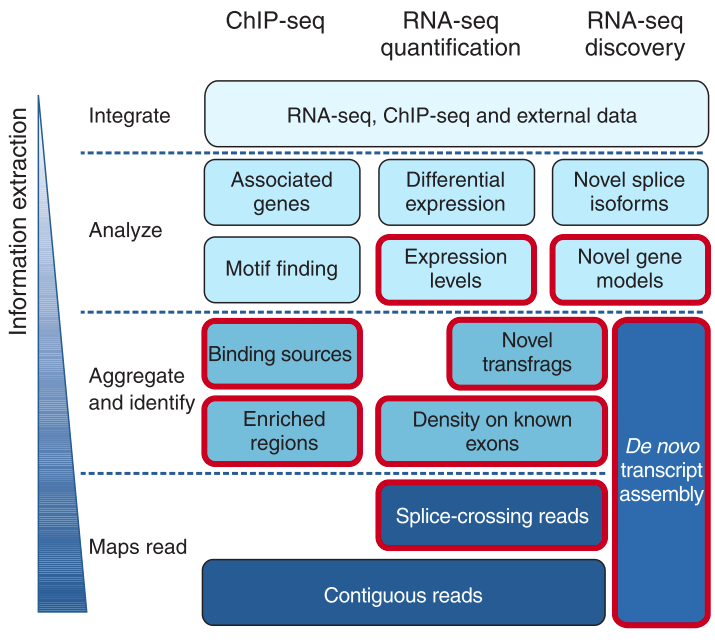
\includegraphics[width=9cm, keepaspectratio]{img/intro/rna-seqan.png}
\caption[RNA-seq analysis]{Representation of \textit{RNA-seq} analysis complexity. \cite{Pepke2009}}
\label{fig:rnaseqan}
\end{figure}

% Due to the widespread of  \textit{RNA-seq} technology the bioinformatics community contributed with several methods for its analysis. 
% Indeed, when working with this data the number of already developed and available methods is so high that for a non-expert user is really easy to understand where to start.

In particular we focused on differential gene expression in case of multiple biological conditions, due to stress, drug treatments, disease-specific, etc. In this specific context, a typical analysis starts from the alignment of the reads on a species's reference genome, followed by the quantification of the mapped reads, producing a count matrix of the samples (on columns) and the genes related features (on the rows), typically identifiers depending on the annotation database used by the analyzer.
Commonly, the count matrix needs to be filtered from low expressed features and then normalized across the samples, to reduce specific bias for each sample.
Then, it is possible to choose between several methods for the detection of differential expression of the features between the conditions (see section \ref{sec:ticorsermethods}).
Finally, the significant features can be integrated with databases of biological functionalities in order to detect the mostly influenced ones.

